\chapter{Future Work}
\label{ch:future}


\section{Anticipated TR WPT System}
\label{sec:future-roadmap}
\todo{Let's think of a better name!}

This research represents a first step in the exploration of building a
time reversal WPT system.
%
We demonstrate one possible realization of this idea in Fig.~\ref{fig:SysImage}.
%
However, we leave optimization of performance and efficiency to future work.


The proposed system consists of two basic components.
%
The first is a rectenna that serves as the receiver.
%
Although the system as described in Section~\ref{sec:meth} would require an
out-of-band feedback channel between the receiver and transmitter, prior work
has shown how a transmitter can target receivers entirely
in-band~\cite{nltr-wave-chaotic,roman}.
%
Our system in Fig.~\ref{fig:SysImage} builds on these findings.
%
The second is a transmitter that performs the time reversal process.
%
This component is responsible for recording characteristic signals from the
receiver(s), time reversing the signals, and re-broadcasting them into the
environment.



In a practical system, the rectenna could be integrated into the hardware of a
mobile device, or into an external component that plugs into the battery.
%
The transmitter would need to be connected to an external power source, but
could otherwise be located anywhere in the room.


Although not a component of the system, another important consideration in this
scenario is the environment; a low-loss scattering environment is necessary for
time reversal to be effective.

\begin{figure}[t]
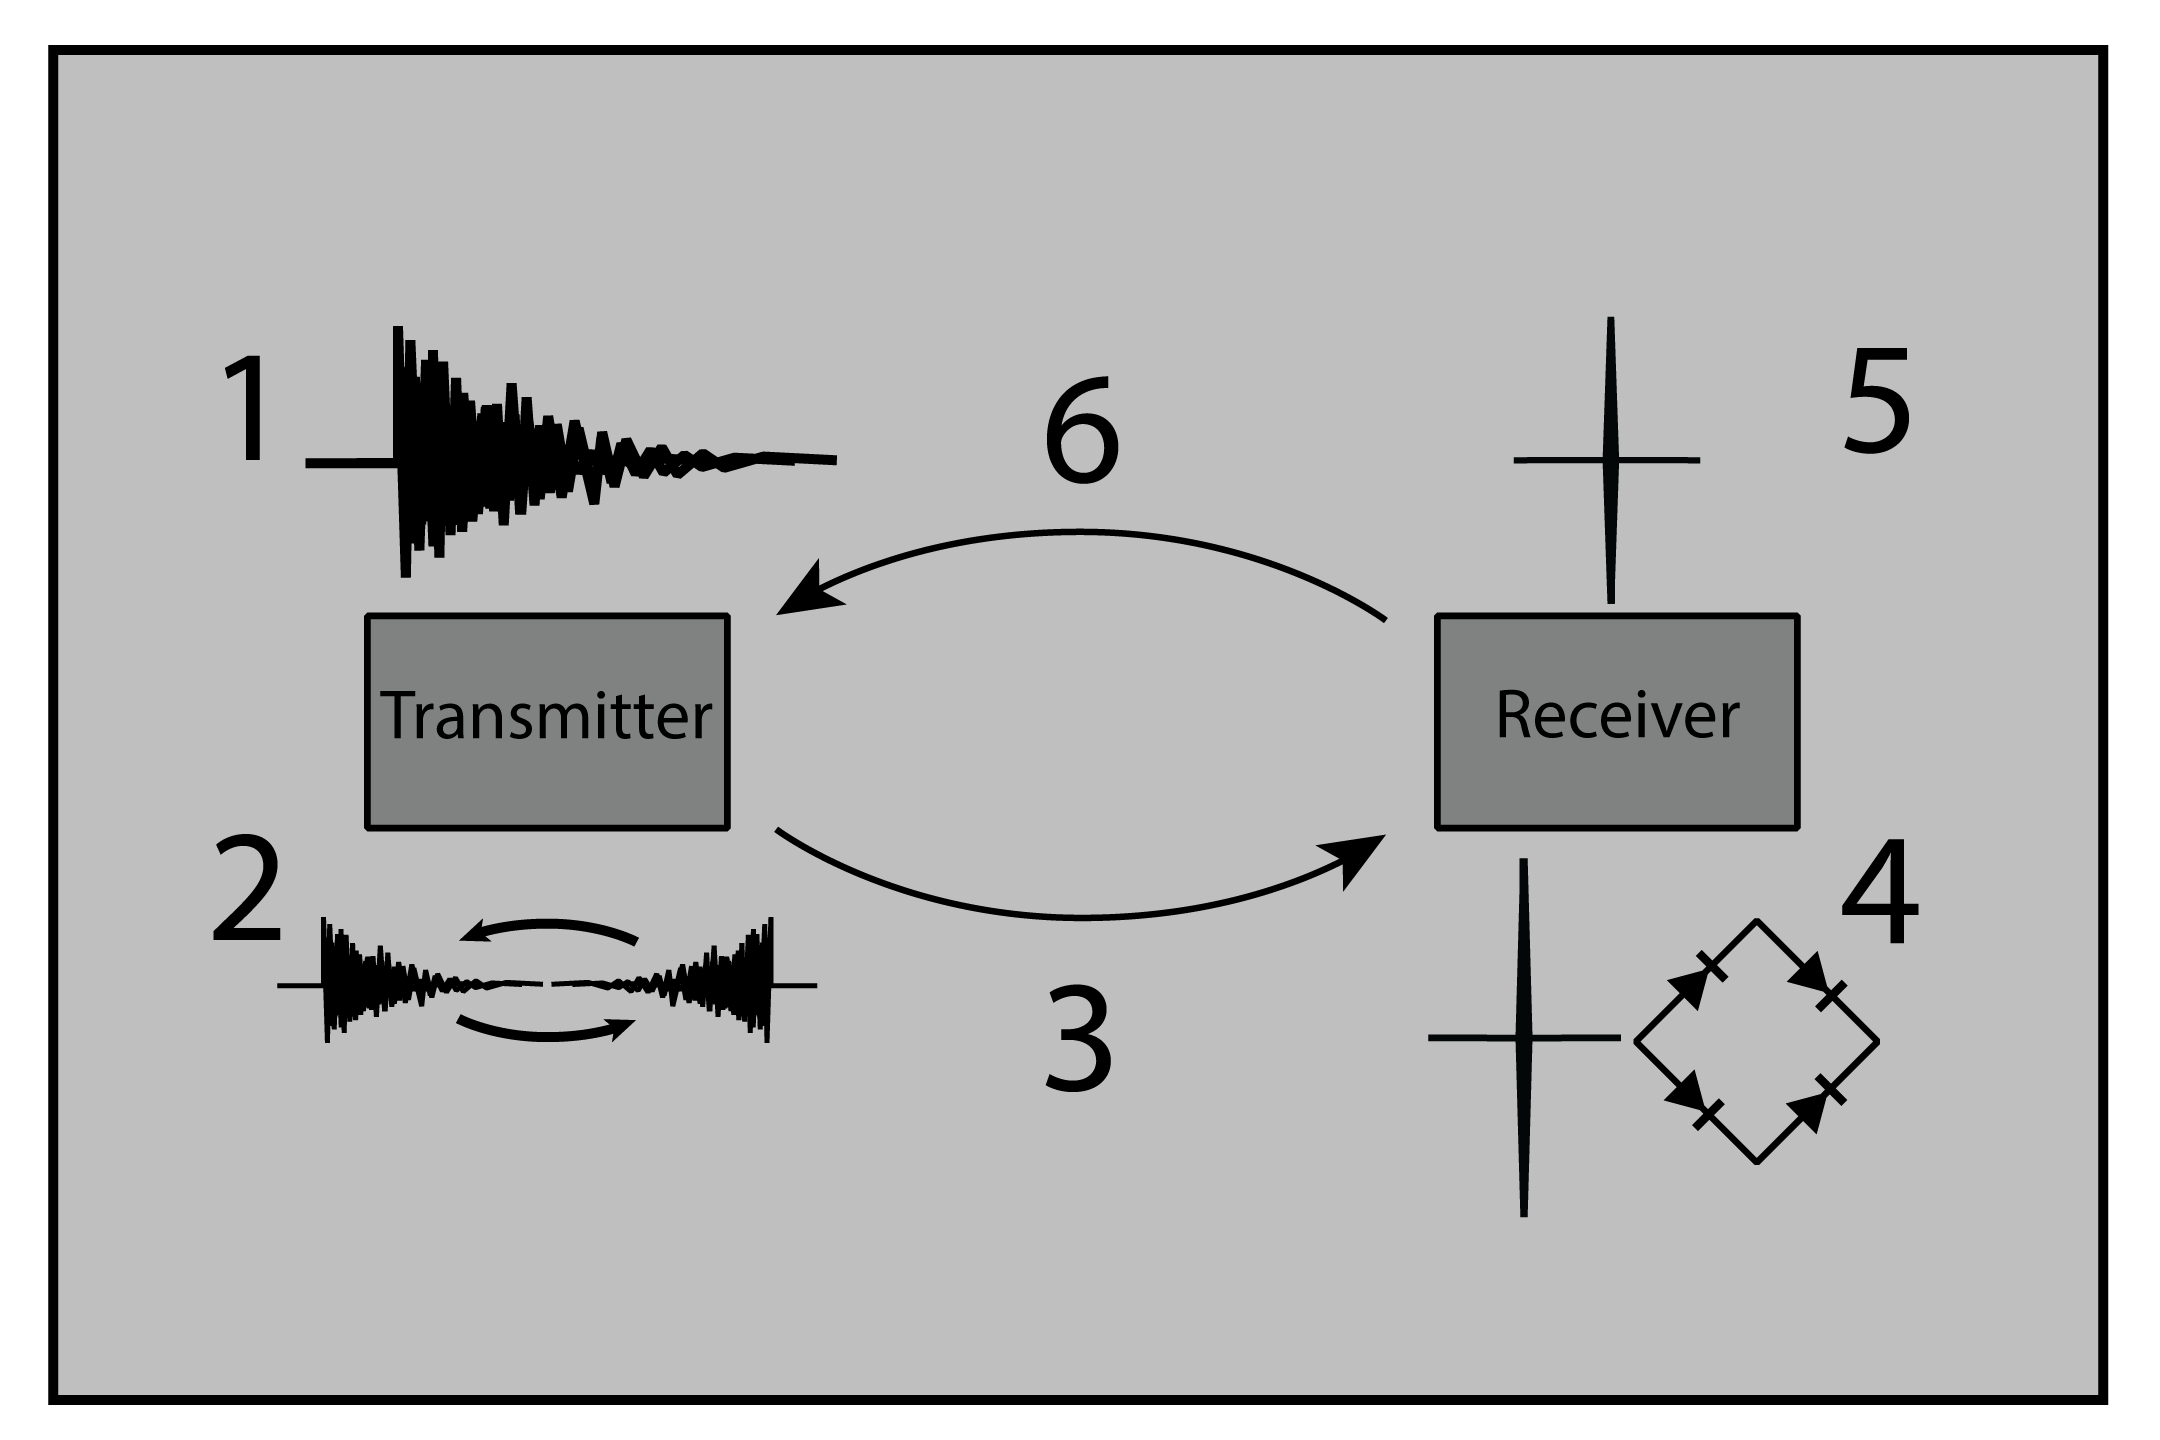
\includegraphics[width=\columnwidth]{figs/future/WPTSys}
\caption{A notional time reversal WPT system. In the acquistion phase, a new receiver joins the system by broadcasting or emitting a characteristic signal (0). Here, the receiver actively emits a signal, but it is also possible for the transmitter to find a passive target, as shown in~\cite{nltr-wave-chaotic}. In either case, the next sona that the transmitter collects will contain spatial information unique to the receiver's location (1). In the power transfer cycle, the sona is time reversed (2), amplified, and broadcast back into the environment. The amplified signal reconstructs on the receiver (3) and is converted to usable DC power by the rectifier (4). A small fraction of the signal is used to re-broadcast a new characteristic signal (5) into the environment, which will be collected in the next sona (6). The cycle repeats from (2).}
\label{fig:SysImage}
\end{figure}



\section{Future work on applying other techniques from TR to WPT}
\label{sec:future-tr}

\subsection{Iterations}

Stuff

\subsection{Multiple Receivers}

Stuff

\subsection{Expontential Amplification}

Stuff
\section{New problems that arise with TR in a WPT context}


\label{sec:future-wpt}

\subsection{Sub Cavity}

Stuff

\subsection{That other thing}

Stuff

\subsection{Timing Analysis}

Stuff
